\documentclass[tikz,border=2pt]{standalone}
\usepackage{amsmath,amssymb}
\usetikzlibrary{arrows.meta}
\begin{document}
% Two equally frequent classes with conditional rates E[Lambda | L=l] = 0.1 and 0.3 (frequency scale, left axis);
% dividing by the base rate 0.2 = E[Lambda] = E[r_L] gives the relativities 0.5 and 1.5 (right axis).
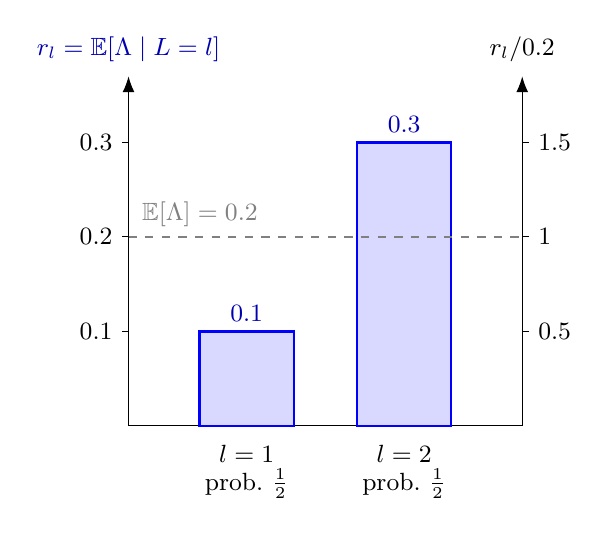
\begin{tikzpicture}[font=\small, >={Latex[length=2mm]}, x=1cm, y=12cm]
  % axes
  \draw[->] (0,0) -- (0,0.37);
  \draw[->] (5,0) -- (5,0.37);
  \draw (0,0) -- (5,0);
  \foreach \v/\r in {0.1/0.5, 0.2/1, 0.3/1.5} {
    \draw (0,\v) -- (-0.08,\v) node[left] {$\v$};
    \draw (5,\v) -- (5.08,\v) node[right] {$\r$};
  }
  \node[anchor=south, blue!70!black] at (0,0.375) {$r_l=\mathbb E[\Lambda\mid L=l]$};
  \node[anchor=south] at (5,0.375) {$r_l/0.2$};
  % bars
  \fill[blue!15] (0.9,0) rectangle (2.1,0.1);
  \draw[blue, thick] (0.9,0) rectangle (2.1,0.1);
  \fill[blue!15] (2.9,0) rectangle (4.1,0.3);
  \draw[blue, thick] (2.9,0) rectangle (4.1,0.3);
  % base rate
  \draw[gray, thick, dashed] (0,0.2) -- (5,0.2);
  \node[gray, anchor=south west] at (0.05,0.2) {$\mathbb E[\Lambda]=0.2$};
  % labels
  \node[blue!70!black, anchor=south] at (1.5,0.1) {$0.1$};
  \node[blue!70!black, anchor=south] at (3.5,0.3) {$0.3$};
  \node[anchor=north, align=center] at (1.5,-0.01) {$l=1$\\[-1pt]prob.\ $\tfrac12$};
  \node[anchor=north, align=center] at (3.5,-0.01) {$l=2$\\[-1pt]prob.\ $\tfrac12$};
\end{tikzpicture}
\end{document}
